\def\widerfacefourk{
    Kế thừa những điểm mạnh như tỷ lệ kích thước, kiểu dáng, biểu cảm, che chắn, góc quay và ánh sáng của bộ dữ liệu WIDER FACE \cite{yang2016wider}, chúng tôi đề xuất một phương pháp xây dựng bộ dữ liệu WIDER FACE 4K gồm có nhiều ảnh có kích thước lớn, giúp đánh giá khách quan độ chính xác và tốc độ của các mô hình giải bài toán nhận diện khuôn mặt.

    \begin{figure}[H]
        \centering
        \subfigure[]{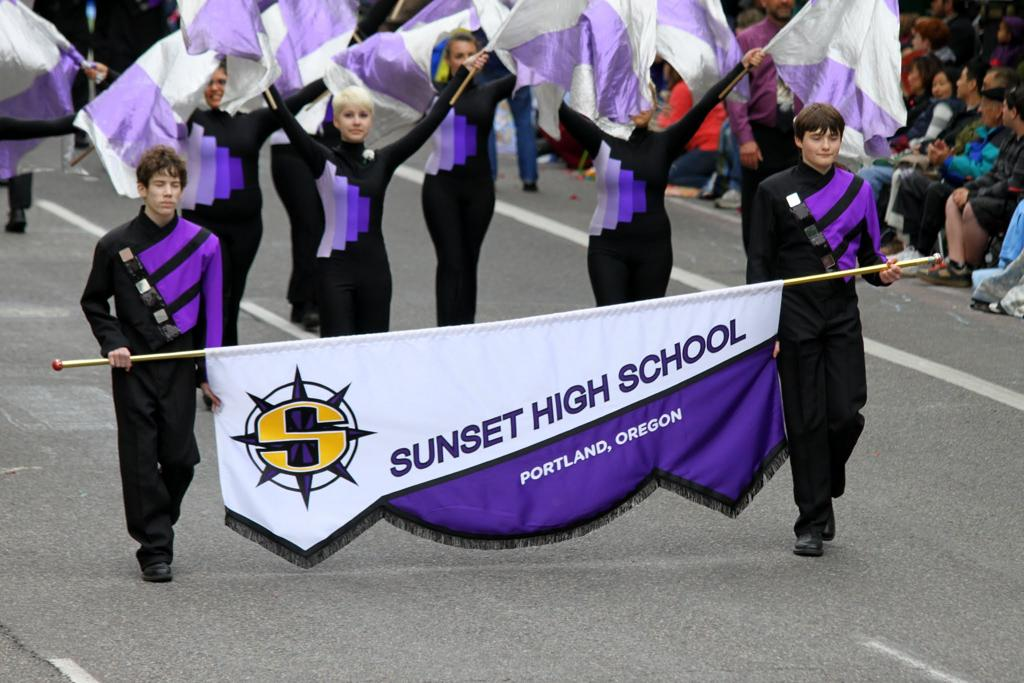
\includegraphics[width=5cm]{images/widerface_highres_1}}
        \subfigure[]{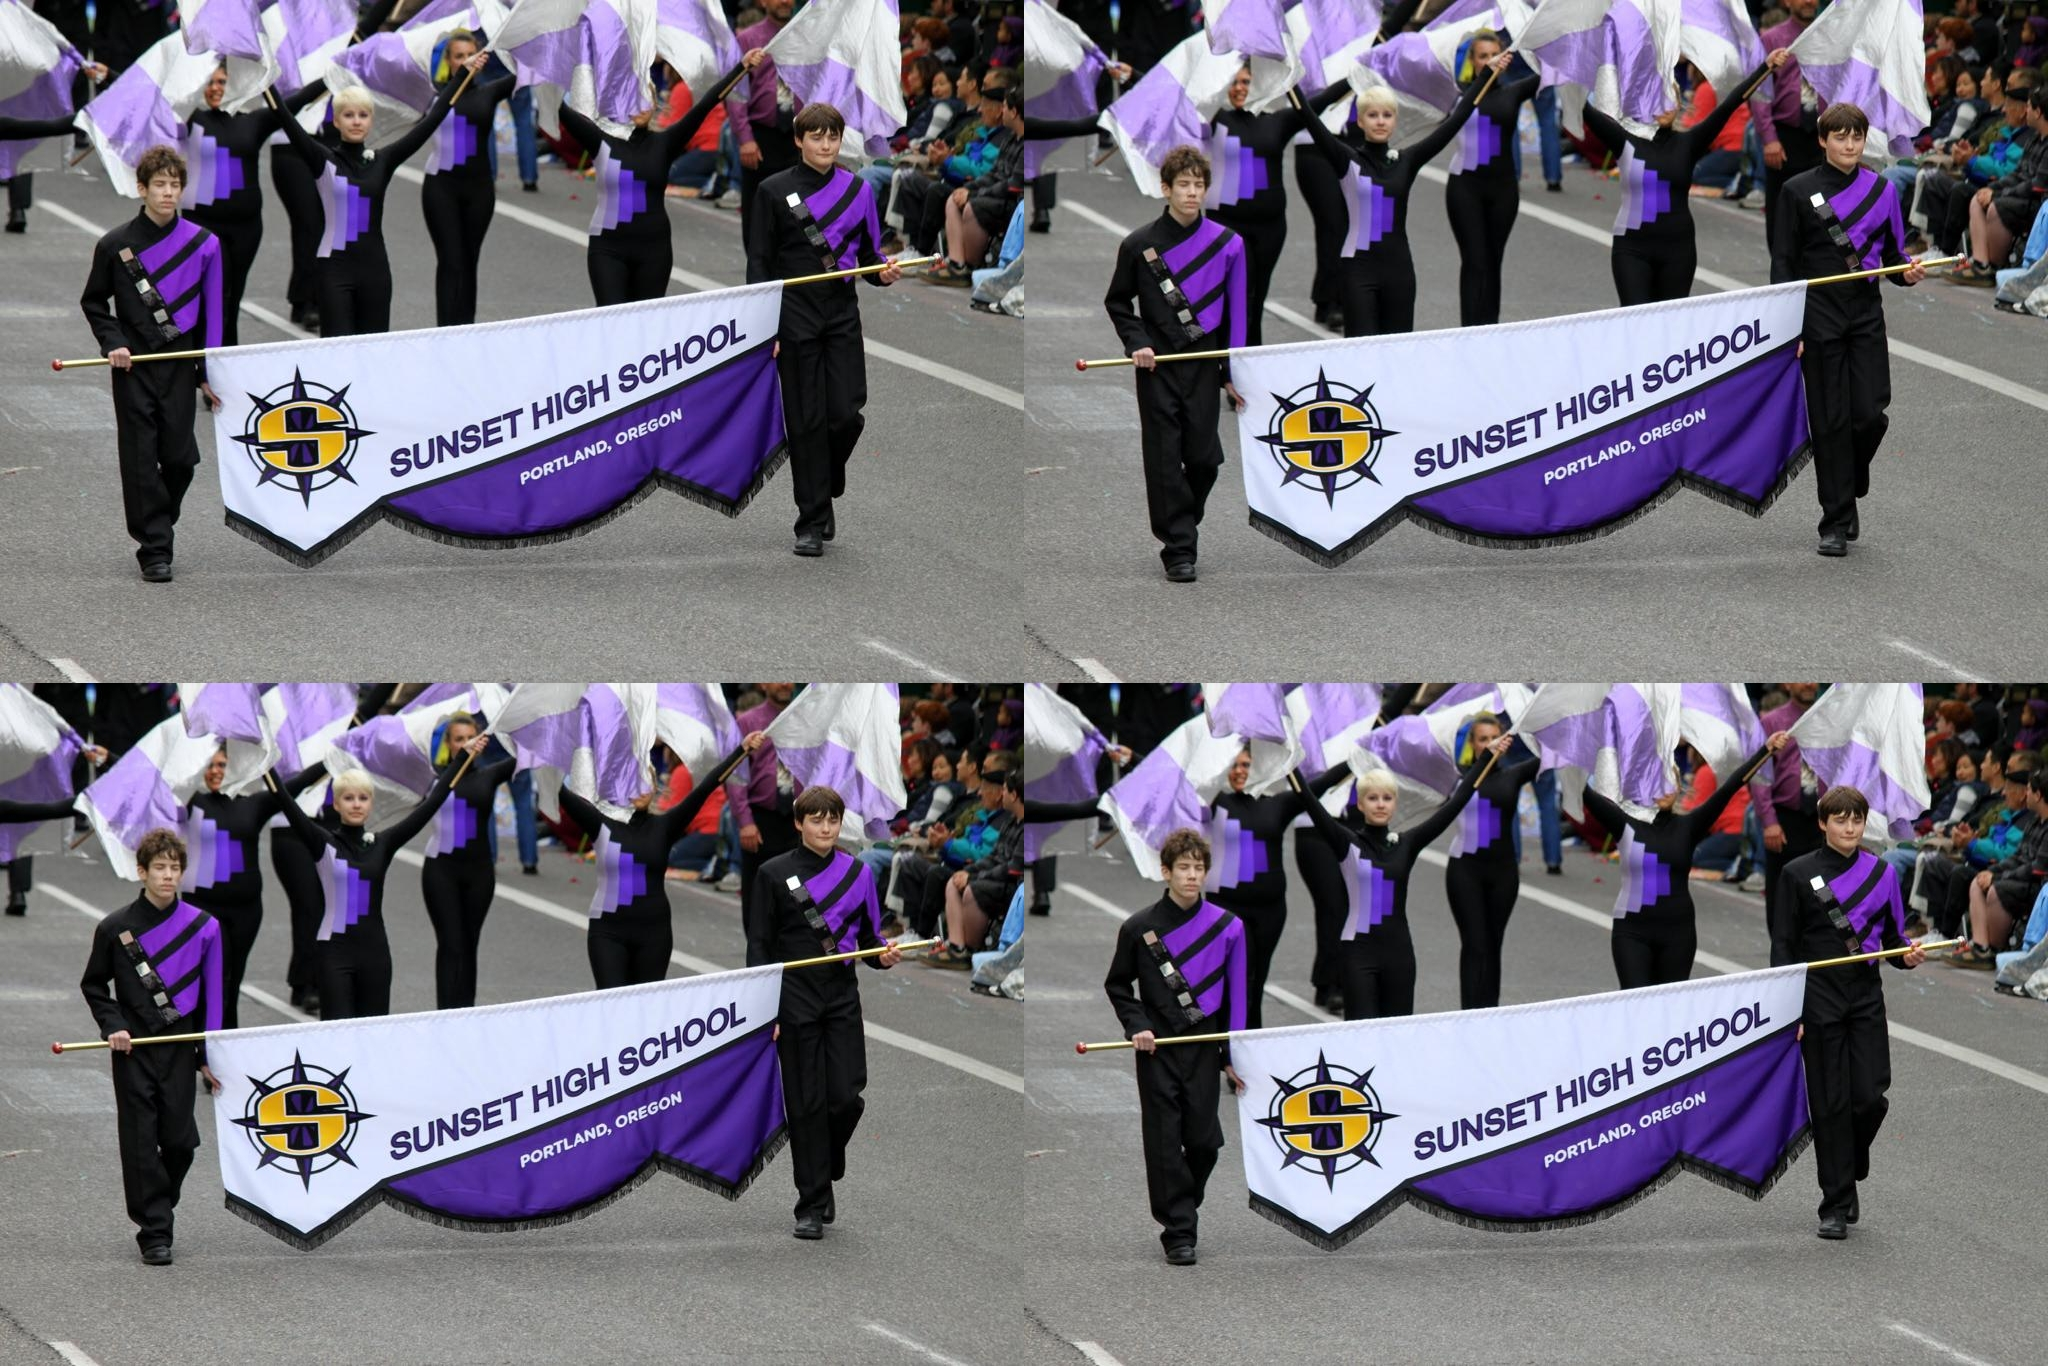
\includegraphics[width=5cm]{images/widerface_highres_2}}
        \subfigure[]{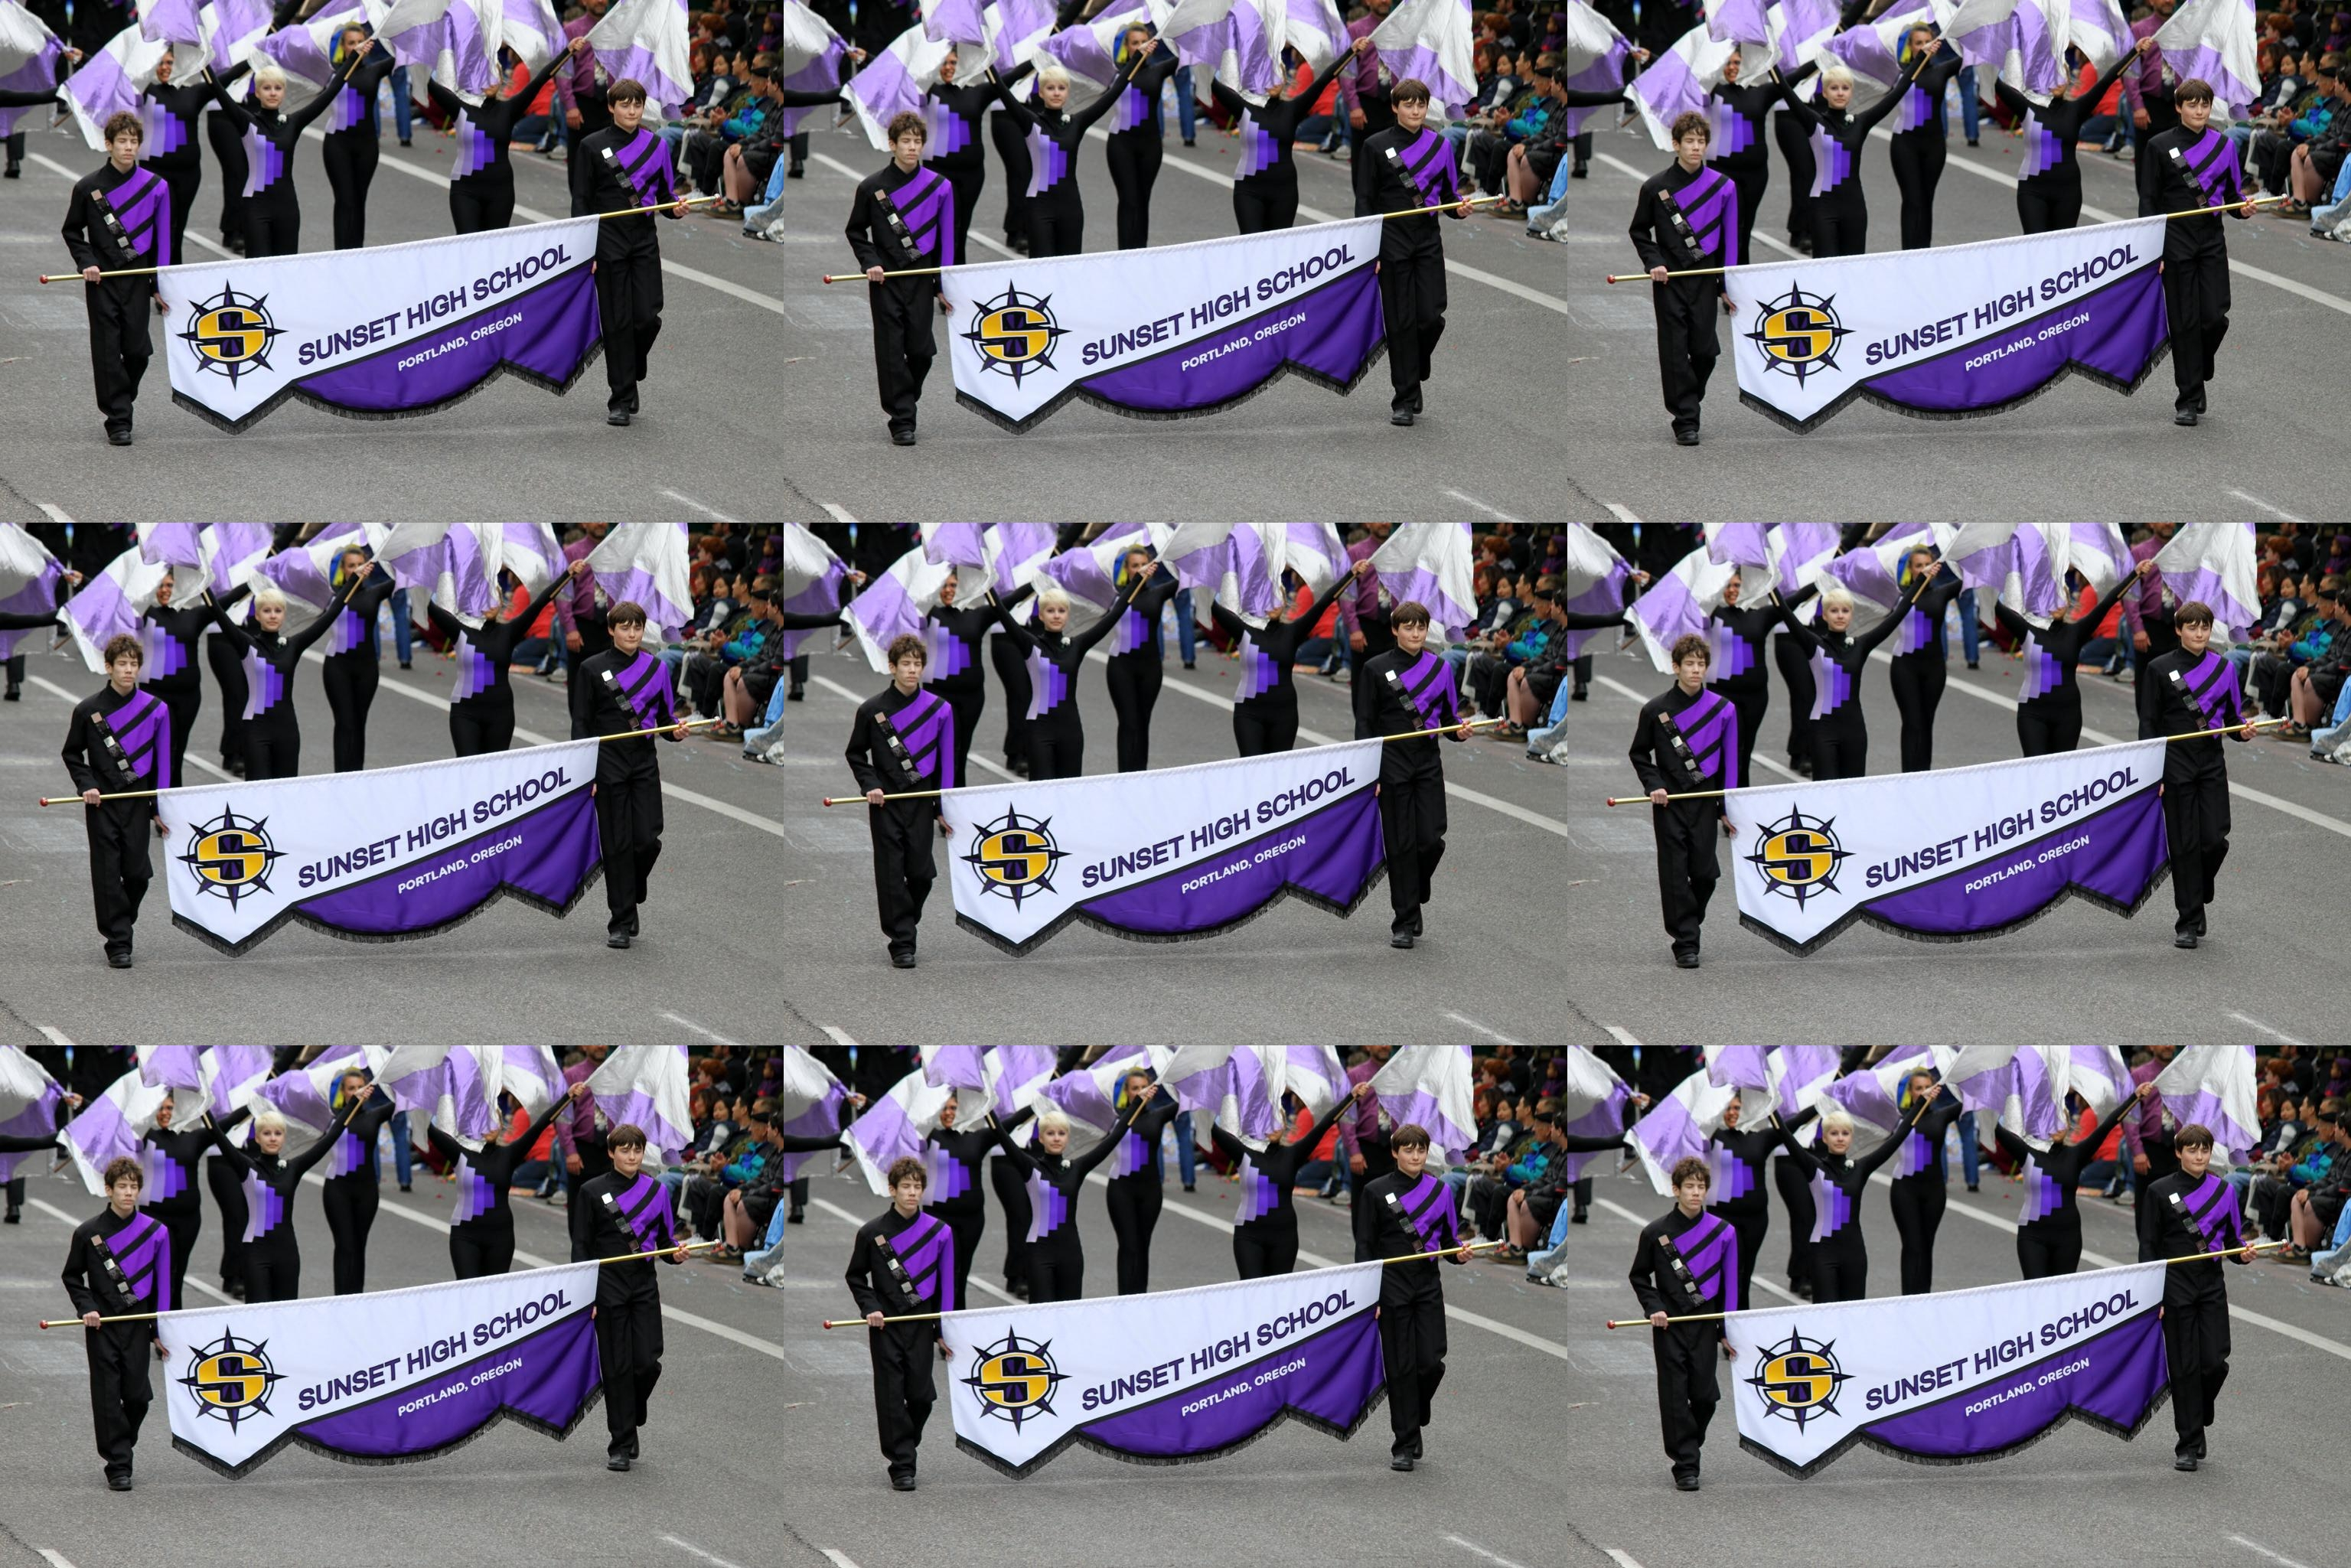
\includegraphics[width=5cm]{images/widerface_highres_3}}
        \subfigure[]{\includegraphics[width=5cm]{images/widerface_highres_4}}
        \subfigure[]{\includegraphics[width=5cm]{images/widerface_highres_5}}
        \caption{Một ví dụ ảnh trong bộ dữ liệu WIDER FACE \cite{yang2016wider} (a) so sánh với bộ dữ liệu WIDER FACE 4K với grid $2 \times 2$ (b), $3 \times 3$ (c), $4 \times 4$ (d) and $5 \times 5$ (d)}
        \label{fig:widerface_4k_example}
    \end{figure}
    
}